\subsection{Analysis by Gender}
\label{analysis by gender}
% summarize and compare the results by gender
% This paper may have something interesting regrading gender \urls{https://ieeexplore.ieee.org/document/9206232}
% \urls{https://ieeexplore.ieee.org/document/7965425}

\bf{In our survey, 90.1\% of participants were male, and 9.9\% participants were
female, which is slightly better than the Stack Overflow (SO) survey
\citep{StackoverflowSurvey2017,StackoverflowSurvey2018,StackoverflowSurvey2019,StackoverflowSurvey2020}
(in Stack Overflow 8\% respondents marked them as female).} It is often said that
females are less represented in STEM. As the SE industry is directly related to
STEM, the claim may be true in the SE industry. Though our survey does not
represent the real scenario, the proportion of male and female participants
supports the claim of under-representation. To get an overview of the Bangladesh
SE industry by gender in Figure \ref{fig:gender and role}, we plotted the
participants' roles grouped by gender.
\begin{figure}[h] \centering
 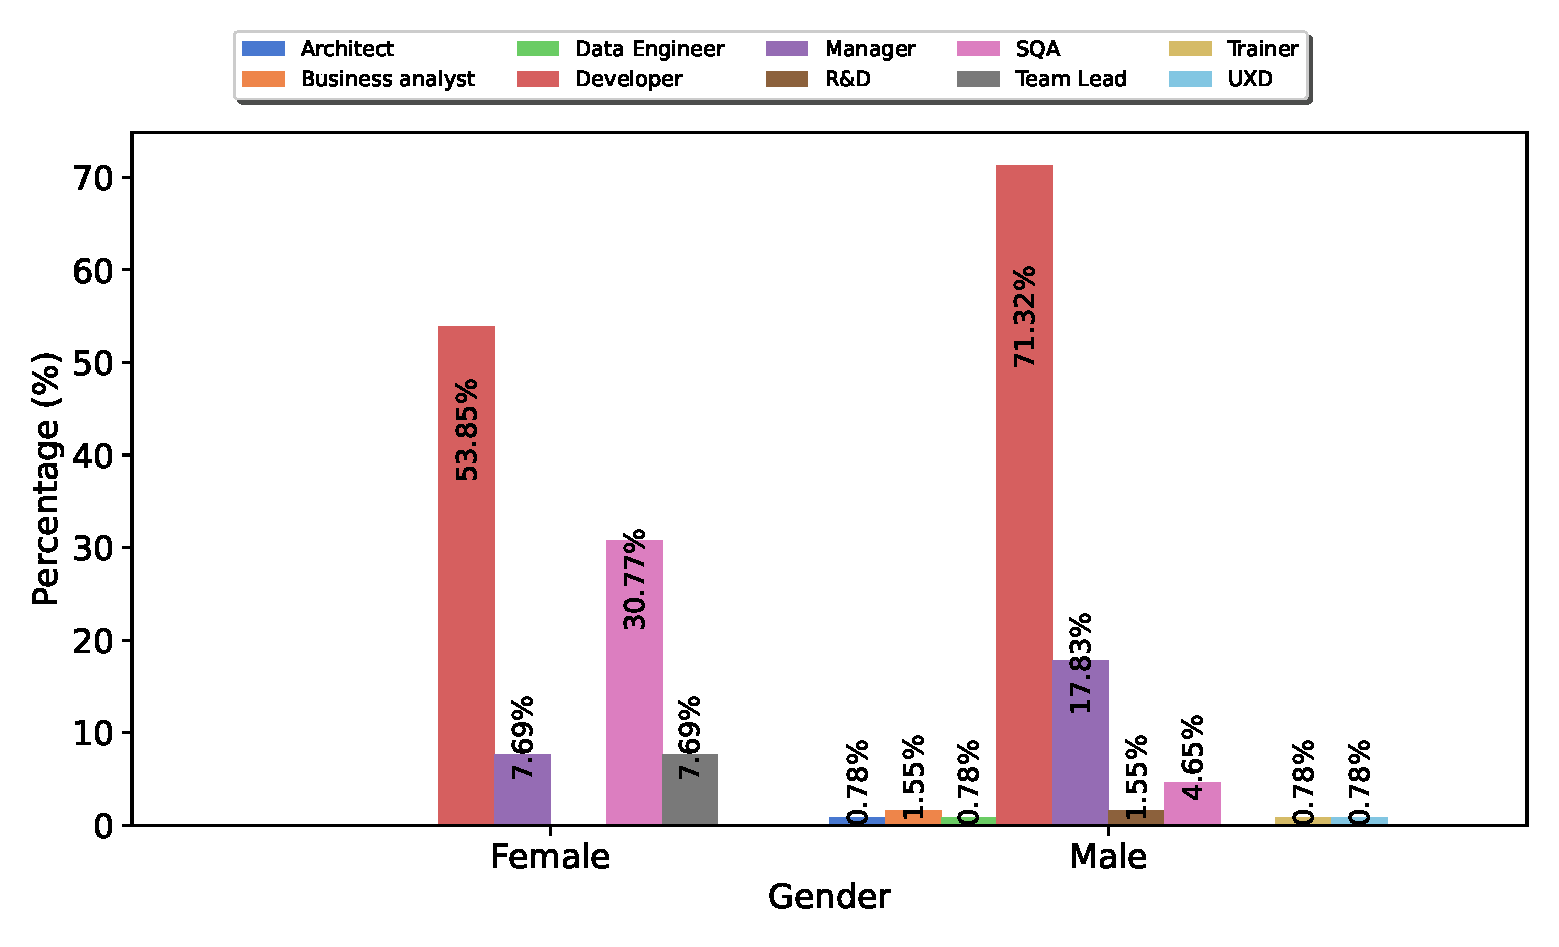
\includegraphics[scale=0.4]{Figures/Gender_and_Role}
 \caption{Gender based role}
 \label{fig:gender and role}
\end{figure}
\bf{In terms of roles, the proportion of developers among female participants is
comparatively low than that of male participants. However, the scenario is the
opposite of the manager and team lead role.} Generally, the developer role is
considered a junior role, and the manager/team lead is considered a senior role.
Thus, it is clear from Figure \ref{fig:gender and role} that there is a
difference between junior and senior roles among female participants. This
indicates that in recent years females are less interested in joining the SE
industry. \bf{Also, among ten different roles, female participants are holding only
four types of roles. Our findings align with the survey result of Hussain et
al.\citep{Hussain2020}. They found that female participants are only limited to
developer, QA, and project manager roles, where male participants are holding
varying types of roles in the Bangladesh SE industry. The result of the Stack
Overflow survey\citep{StackoverflowSurvey2020} is slightly different. In the SO
survey, female respondents are mostly data scientists, business analysts, QA,
and developer roles. A common theme in all surveys is the role of female
respondents in the QA.}

\newcolumntype{b}{X}
\newcolumntype{v}{>{\hsize=.03\hsize}X}
\newcolumntype{m}{>{\hsize=.2\hsize}X}
\newcolumntype{y}{>{\hsize=.33\hsize}X}
\begin{table}[htbp]
    \centering
    \caption{Highlights of Findings from Survey Closed Questions by Gender}
    \begin{tabularx}{\textwidth}{v|b}
        \hline
        \textbf{No}     & \textbf{Question}  \\ \hline
        2 & What is your age?\newline
        1) 15 to 20: \textbf{\textit{Male, 100.0\% } } 2) 20 to 25: \textbf{\textit{Male, 87.8\% } } 3) 25 to 30: \textbf{\textit{Male, 86.84\% } } 4) 30 to 35: \textbf{\textit{Male, 96.0\% } } 5) 35 to 40: \textbf{\textit{Male, 100.0\% } } 6) 40 to 45: \textbf{\textit{Male, 100.0\% } } \\ \hline
        4 & For how many years have you coded professionally?\newline
        1) less than 2: \textbf{\textit{Male, 89.13\% } } 2) 2 to 5: \textbf{\textit{Male, 91.18\% } } 3) 5 to 10: \textbf{\textit{Male, 80.77\% } } 4) more than 10: \textbf{\textit{Male, 100.0\% } } \\ \hline
        5 & What is your current role?\newline
        1) Architect: \textbf{\textit{Male, 100.0\% } } 2) Business analyst: \textbf{\textit{Male, 100.0\% } } 3) Data Engineer: \textbf{\textit{Male, 100.0\% } } 4) Developer: \textbf{\textit{Male, 92.93\% } } 5) Manager: \textbf{\textit{Male, 95.83\% } } 6) R\&D: \textbf{\textit{Male, 100.0\% } } 7) SQA: \textbf{\textit{Male, 60.0\% } } 8) Team Lead: \textbf{\textit{Female, 100.0\% } } 9) Trainer: \textbf{\textit{Male, 100.0\% } } 10) UXD: \textbf{\textit{Male, 100.0\% } } \\ \hline
        6 & Which of the following software development methodologies do you follow?\newline
        1) Agile: \textbf{\textit{Male, 86.36\% } } 2) Kanban: \textbf{\textit{Male, 100.0\% } } 3) Others: \textbf{\textit{Male, 100.0\% } } 4) Pair Programming: \textbf{\textit{Male, 96.43\% } } 5) Scrum: \textbf{\textit{Male, 93.75\% } } 6) Waterfall: \textbf{\textit{Male, 100.0\% } } 7) XP: \textbf{\textit{Female, 100.0\% } } \\ \hline
        9 & Which of the following technologies do you have experience working in?\newline
        1) Cloud: \textbf{\textit{Male, 100.0\% } } 2) Desktop: \textbf{\textit{Male, 78.57\% } } 3) Embedded /IOT: \textbf{\textit{Male, 100.0\% } } 4) Mobile: \textbf{\textit{Male, 90.62\% } } 5) Others: \textbf{\textit{Male, 100.0\% } } 6) Web: \textbf{\textit{Male, 90.0\% } }\\ \hline
    \end{tabularx}
    \label{table:analysis by gender}
\end{table}

The interesting findings of gender analysis are presented in Table
\ref{table:analysis by gender}. James et al.'s \citep{James2017} survey on male
and female software professionals found that men are more likely to be in senior
positions than women. In Q4 of Table \ref{table:analysis by gender}, we observe
a similar scenario. However, in our case, the observation is not statistically
significant. \bf{James et al. \citep{James2017} also found that male software practitioners tend to be older
than female practitioners and female practitioners tend to leave jobs in
mid-career. We observe the same phenomena in Q2 and Q4, and the finding may be
true in Bangladesh.}


James et al.\citep{James2017} found that female practitioners express less
satisfaction with the spirit of teamwork inside the organization. They conclude
that this characteristic would make male practitioners a key part of a good
agile team. Our findings differs from James et al. \citep{James2017}. In Q6 of
Table \ref{table:analysis by gender}, we observe that our survey's female
participants prefer the Agile methodology over other software development
methodologies. However, development methodology selections are often performed
by senior management. Thus, personal preferences can have minimal effect on this
choice

In James et al. \citep{James2017} survey, neither male nor female was not dominating any
particular technology field. However, in Q9 of Table \ref{table:analysis by
gender} we observe female participants working on desktop, web, and mobile. As a
small SE industry, cloud/IoT is considered a less secured field as job
opportunities in these fields are small. It seems female participants tend to
work in a more secure technology (in terms of a job opportunity) field.